%%===============================================================
%%===============================================================
\chapter{Pre-processor}
%%===============================================================
%%===============================================================
%%===============================================================
% Authors: Valentin Zingan, Chad Balen,
%          Mayank Sabharwal, Aslan Kosakian (editing)
%%===============================================================

In order to generate a fuel cell domain using OpenFCST, two options are available:
\begin{itemize}
 \item use the classes under \texttt{FuelCell::Geometry} namespace;
 \item read in a mesh generated with an open-source mesh generator such as SALOME.
\end{itemize}

OpenFCST also allows you to generate VTK meshes from stacks of images obtained with FIB-SEM, TEM, etc. This functionality is available through PythonFCST, a Python extension of OpenFCST.

%%===============================================================
\section{\texttt{FuelCellShop::Geometry} Namespace}
Namespace \texttt{FuelCellShop::Geometry} contains classes to generate a cathode and anode fuel cell electrodes and a membrane electrode assembly with five or seven layers (i.e. with and without microporous layer). To use these classes, you simply need to create an object of the class. Then, use the \verb!declare_parameters! member function to define the variables required in the input file, initialize the object calling \verb!initialize! and generate the grid using \verb!generate_grid!. For example,
\begin{lstlisting}
//Create object
FuelCellShop::Geometry::PemfcMPL<dim> grid; 
//Declare the necessary variables in the ParameterHandler deal.ii object
grid.declare_parameters(param);         
//Once the ParameterHandler object has been initialized by reading from file, 
//initialize the geometry varialbes 
grid.initialize(param);                 
//Generate the mesh and store it in the dealii::Triangularization variable tr  
grid.generate_grid(*this->tr);          
\end{lstlisting}

You can use some pre-defined geometry templates using OpenFCST GUI or the parameter files. The list of options available for the \texttt{FuelCellShop::Geometry::GridBase} class is as follows:
\begin{itemize}
\item \textbf{GridExternal} - import external mesh;
\item \textbf{Cathode} - catalyst and gas diffusion layers on the cathode side;
\item \textbf{Anode} - catalyst and gas diffusion layers on the anode side;
\item \textbf{CathodeMPL} - same as \textbf{Cathode}, but with a microporous layer;
\item \textbf{Pemfc} - combines \textbf{Cathode} and \textbf{Anode} and adds a polymer electrolyte membrane inbetween;
\item \textbf{PemfcMPL} - same as \textbf{Pemfc}, but with micropurous layers on both cathode and anode sides.
\end{itemize}

%%===============================================================
\section{Developing a mesh in SALOME}
SALOME is an open-source cross-platform software that provides a generic platform for pre-processing. It is distributed under the terms of the GNU LGPL license. You can download both source code and executable files from the \htmladdnormallink{SALOME website}{http://www.salome-platform.org/}.

%%=======
\subsection{Tutorial}
This short tutorial demonstrates how to create a simple mesh in Salome 7.3.0, define material and boundary indicators, and adapt all of this to the needs of OpenFCST.

The object we would like to mesh is represented by a two dimensional H-shaped domain as shown in Figure~\ref{fig:no3.2.1.1}.

\begin{figure}[h!]
\begin{center}
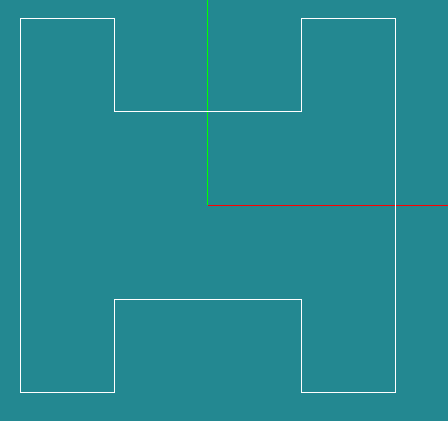
\includegraphics[width=0.43\textwidth]{figures/salome0.png}
\caption{H-shaped domain.}
\label{fig:no3.2.1.1}
\end{center}
\end{figure}

OpenFCST only accepts meshes composed of either quadrilaterals in 2D or hexahedrals in 3D. \textbf{OpenFCST assumes that all the geometrical dimensions are in centimeters}. The current version of Salome is only able to produce these type of meshes with geometries that have an outer boundary composed exactly of 4 pieces in 2D, e.g. see Figure~\ref{fig:no3.2.1.2}, and 6 pieces in 3D, e.g see Figure~\ref{fig:no3.2.1.3}. In order to increase the quadrilateral and hexahedral properties of Salome however, a commercial package called Hexotic is distributed by Distine (for more information, please visit the \htmladdnormallink{site}{http://www-roc.inria.fr/gamma/gamma/Membres/CIPD/Loic.Marechal/Research/Hexotic.html}).

\begin{figure}[h!]
\begin{center}
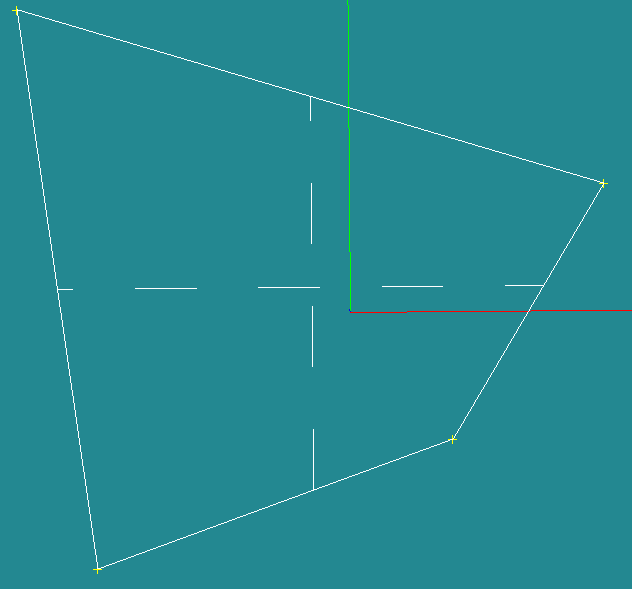
\includegraphics[width=0.43\textwidth]{figures/salome01.png}
\caption{Linear quadrilateral.}
\label{fig:no3.2.1.2}
\end{center}
\end{figure}

\begin{figure}[h!]
\begin{center}
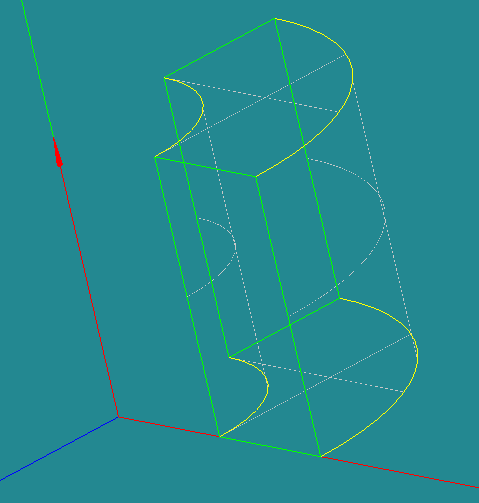
\includegraphics[width=0.43\textwidth]{figures/salome02.png}
\caption{Quarter of cylindrical shell.}
\label{fig:no3.2.1.3}
\end{center}
\end{figure}

The two dimensional H-shaped domain shown in Figure~\ref{fig:no3.2.1.1} has 12 pieces for the outer boundary and hence can not be meshed in Salome directly by means of quadrilaterals. We can mesh the domain however by splitting it into 3 parts, such that each of the parts has 4 outer boundary segments. Then, we mesh each of these parts and combine them into the H-shaped domain.

Let us do this step by step.

\subsubsection{Creating a geometric entity}

Run Salome, select \textbf{New document}, and then select \textbf{Geometry} on the upper toolbox (Figure \ref{fig:no3.2.1.4}). 

\begin{figure}[h!]
\begin{center}
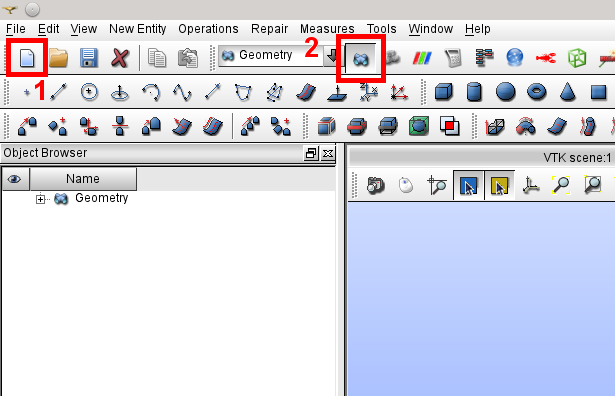
\includegraphics[scale=0.60]{figures/SalomeStep1.png}
\caption{Starting a New Project.}
\label{fig:no3.2.1.4}
\end{center}
\end{figure}
  
We are now in the Geometry module of Salome, and the first thing we need to do is to define 12 vertices along the object: 
\begin{itemize}
 \item 1(-1, -1)
 \item 2(-0.5, -1)
 \item 3(-0.5, 1)
 \item 4(-1, 1)
 \item 5(-0.5, -0.5)
 \item 6(0.5, -0.5)
 \item 7(0.5, 0.5)
 \item 8(-0.5, 0.5)
 \item 9(0.5, -1)
 \item 10(1, -1)
 \item 11(1, 1)
 \item 12(0.5, 1)
\end{itemize}
To create any of these points, we go to \textbf{New Entity} $\rightarrow$ \textbf{Basic} $\rightarrow$ \textbf{Point}, specify a \textbf{Name} and the respective fields \textbf{X:}, \textbf{Y:}, and \textbf{Z:}, then select \textbf{Apply}. For the last vertex use the \textbf{Apply and Close} button instead of Apply. Note that instead of \textbf{New Entity} $\rightarrow$ \textbf{Basic} $\rightarrow$ \textbf{Point} we can simply choose \textbf{Create a point} on the upper toolbox. After initializing all the points select the -OZ view button to change the view and zoom into our geometry (Figure \ref{fig:no3.2.1.5}).

\begin{figure}[h!]
\begin{center}
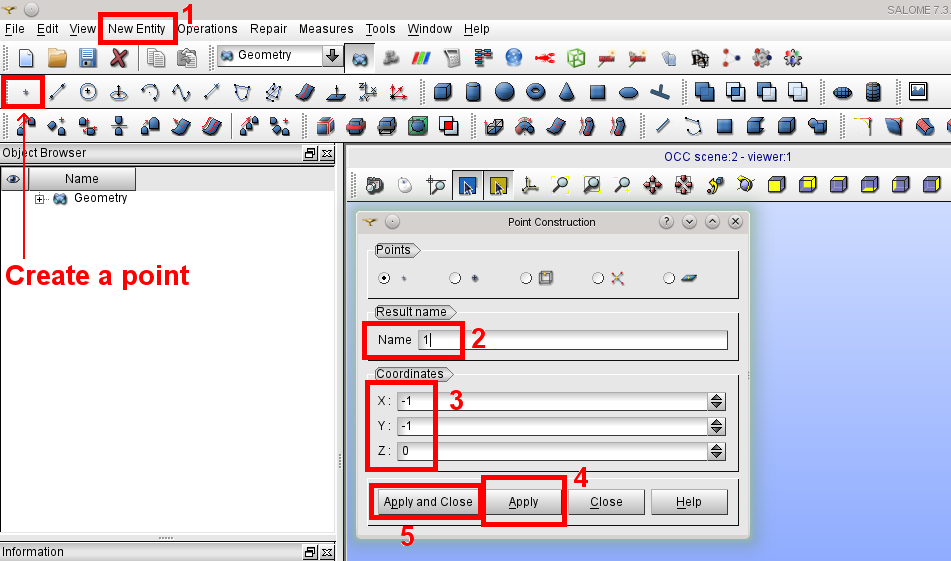
\includegraphics[scale=0.50]{figures/SalomeStep1b.png}
\caption{Creating a Point.}
\label{fig:no3.2.1.5}
\end{center}
\end{figure}

Next we create 3 quadrangle faces. Each of these faces consists of 4 points:
\begin{itemize}
 \item 1(1, 2, 3, 4)
 \item 2(5, 6, 7, 8)
 \item 3(9, 10, 11, 12).
\end{itemize}

To create a quadrangle face, we go to \textbf{New Entity} $\rightarrow$ \textbf{Blocks} $\rightarrow$ \textbf{Quadrangle Face}, fill out the fields \textbf{Vertex 1}, \textbf{Vertex 2}, \textbf{Vertex 3}, and \textbf{Vertex 4} with the points from above, and select \textbf{Apply and Close} button (Figure \ref{fig:no3.2.1.7}). To prevent possible problems always specify vertices in a counter-clockwise direction.

\begin{figure}[h!]
\begin{center}
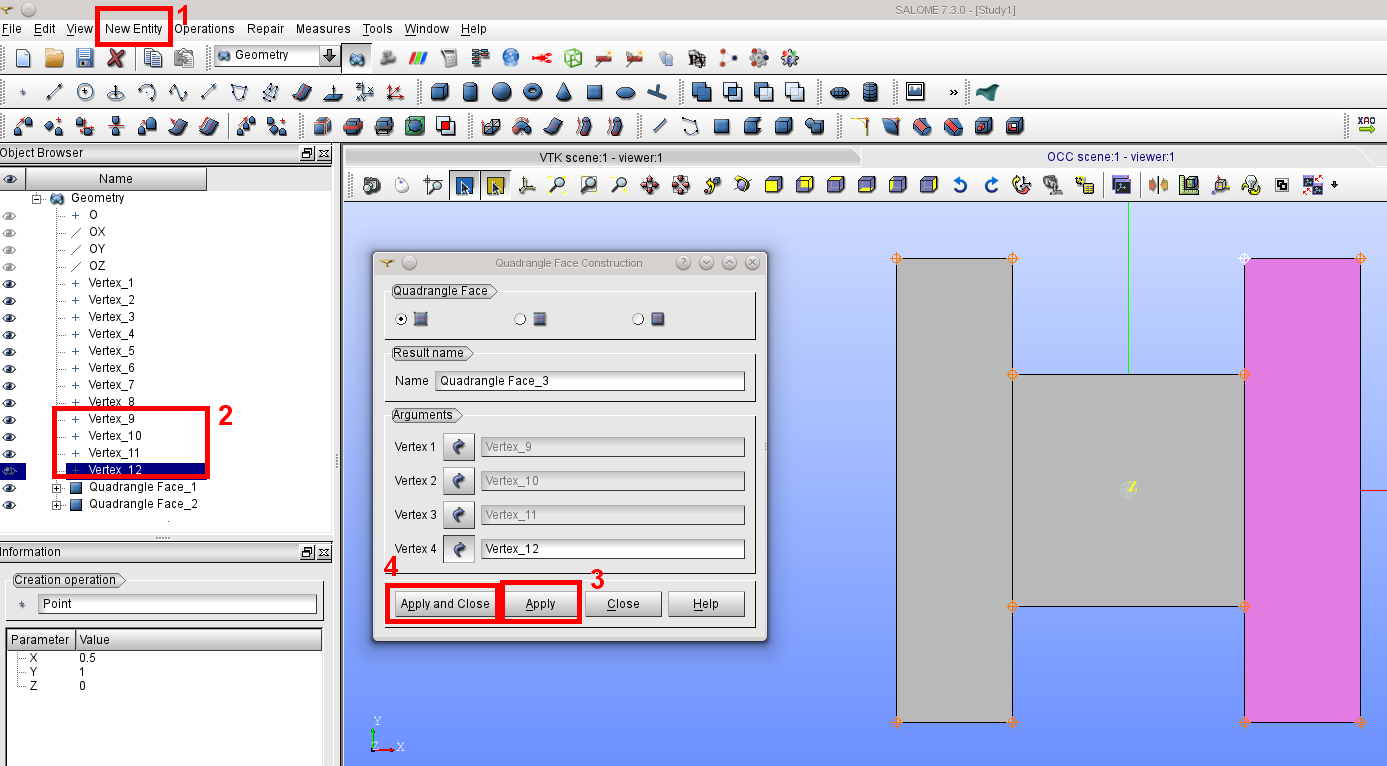
\includegraphics[scale=0.4]{figures/SalomeStep2.png}
\caption{Creating a Quadrangle Face.}
\label{fig:no3.2.1.7}
\end{center}
\end{figure}

\subsubsection{Generating a mesh for each domain}

At this point we have created our geometry. We now would like to generate the mesh. For this, we switch our attention to the Mesh module. To enter the Mesh module, select the \textbf{Mesh} button on the upper toolbox. To create an appropriate mesh on each of the quadrangle faces, we go to \textbf{Mesh} $\rightarrow$ \textbf{Create Mesh}, where we pass the respective quadrangle face to the \textbf{Geometry} field. Once this is done, we select \textbf{Quadrangle (Mapping)} from the drop-down menu of the \textbf{Algorithm} field (Figure \ref{fig:no3.2.1.9}).

\begin{figure}[h!]
\begin{center}
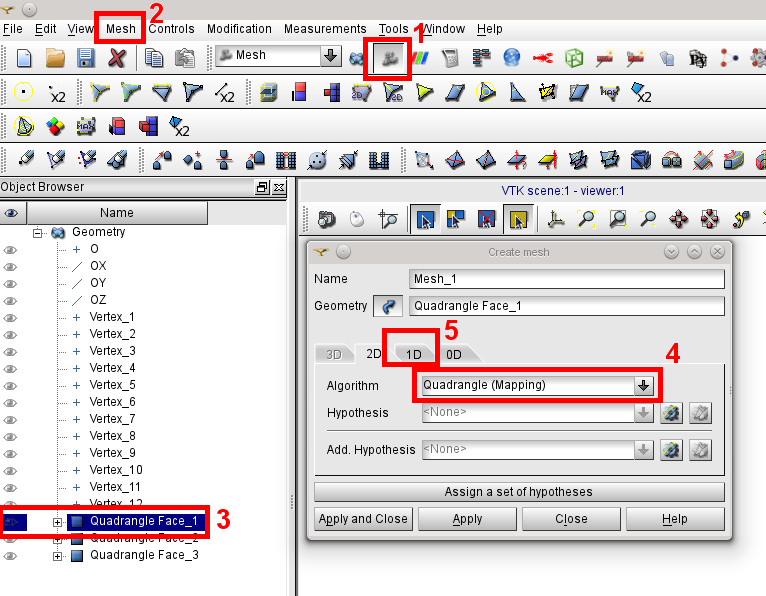
\includegraphics[scale=0.50]{figures/SalomeStep3.png}
\caption{Creating a Mesh.}
\label{fig:no3.2.1.9}
\end{center}
\end{figure}

After that we select the \textbf{1D} tab and check that \textbf{Algorithm} is set up to \textbf{Wire discretization}. The number of 1D hypotheses is available here. We choose the one which is called \textbf{Local Length}. This method uses a uniform spacing between nodal mesh points to generate the mesh on the selected edge. Set the \textbf{Length} parameter to 0.5 as shown in Figure \ref{fig:no3.2.1.10}.

\begin{figure}[h!]
\begin{center}
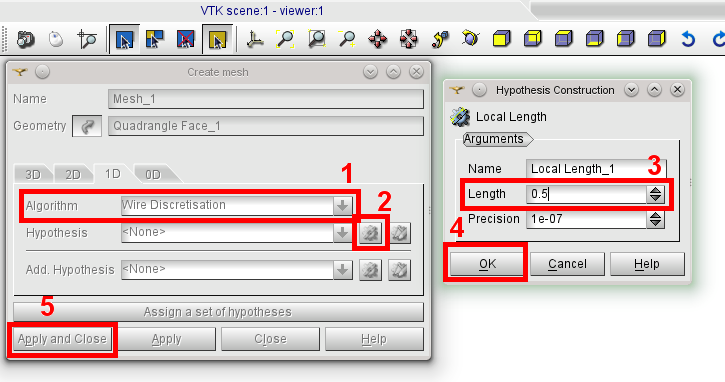
\includegraphics[scale=0.50]{figures/SalomeStep3b.png}
\caption{Setting Mesh Parameters.}
\label{fig:no3.2.1.10}
\end{center}
\end{figure}

After clicking \textbf{OK}, the name of the \textbf{Hypothesis} field should change to \textbf{Local Length\_1}. Then \textbf{Apply and Close}. Right click on the \textbf{Mesh\_1} and \textbf{Compute}. After applying this strategy to all the quadrangle faces and selecting the -OZ view button again, we have something like Figure \ref{fig:no3.2.1.11}.

\begin{figure}[h!]
\begin{center}
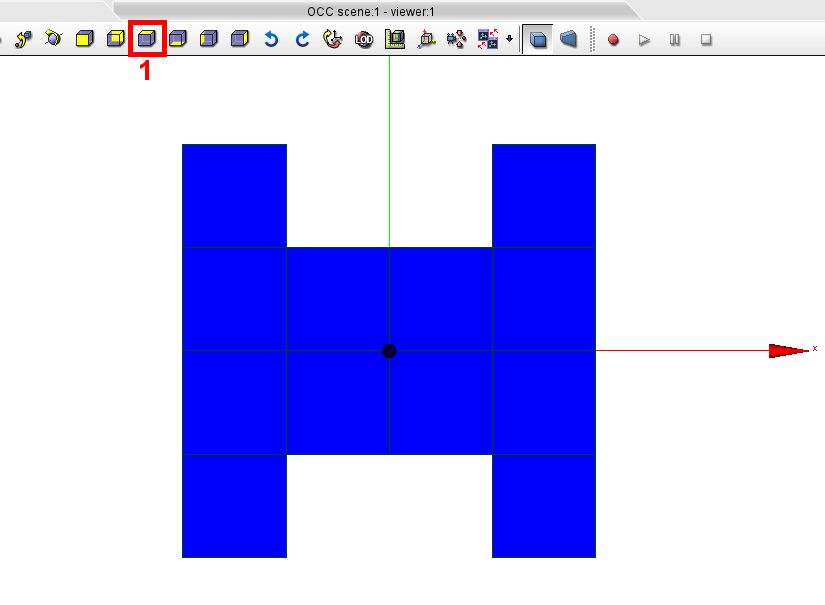
\includegraphics[scale=0.50]{figures/SalomeStep3c.png}
\caption{Overview of the Mesh.}
\label{fig:no3.2.1.11}
\end{center}
\end{figure}

At this point we have generated one mesh for each geometrical entity. These meshes still need to be combined into an overall mesh. Furthermore, we might want to identify each geometrical entity and boundary with an indicator so that we can apply different properties in each domain.

\subsubsection{Assigning material and boundary IDs to different parts of the mesh and creating an overall mesh}

Let us now assign Material IDs to all the cells we have created. \textbf{Material IDs in OpenFCST need to be unsigned integers}, so please do not use names as material IDs. Let us assign all the cells of Mesh\_1 a Material ID = 1, those belonging to Mesh\_2 a Material ID = 2, and cells from Mesh\_3 a Material ID = 3. To assign the material IDs, right click on \textbf{Mesh\_1}, then select \textbf{Create Group}. On this dialog box specify an \textbf{Element Type} of \textbf{Face}, \textbf{Name} of 1,\textbf{Select All}, and finally \textbf{Apply and Close} (Figure \ref{fig:no3.2.1.12}). Repeat this process for the other Material IDs.

\textit{Tip:} If you wish to use the \textbf{Manual Selection} option to add the cells to the \textbf{Id Elements} field, push and hold the Shift key on your keyboard and select the cells by left clicking. After all the desired cells have been highlighted, select \textbf{Add} in the Create Group dialog window.

\begin{figure}[h!]
\begin{center}
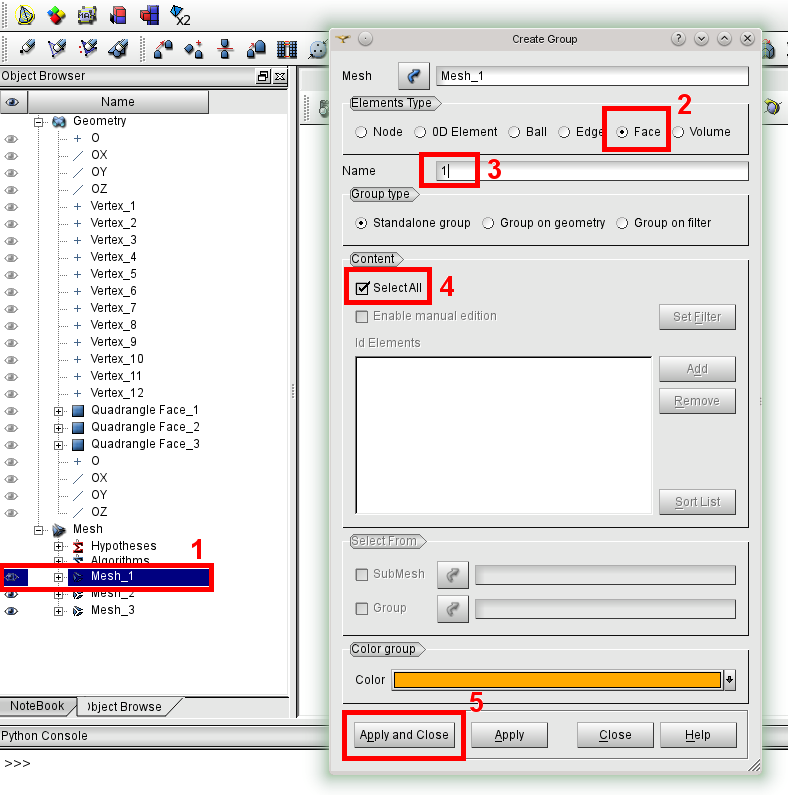
\includegraphics[scale=0.50]{figures/SalomeStep4.png}
\caption{How to Set the Material ID.}
\label{fig:no3.2.1.12}
\end{center}
\end{figure}

Now create a Compound Mesh by simply merging all the previously created meshes. This is done by selecting all the meshes, then from the toolbox \textbf{Mesh} $\rightarrow$ \textbf{Build Compound}. Specify a \textbf{Name}, select \textbf{Create common groups for initial meshes} and \textbf{Merge coincident nodes and elements}, and finally select \textbf{Apply and Close} (Figure \ref{fig:no3.2.1.13}).
        
\begin{figure}[h!]
\begin{center}
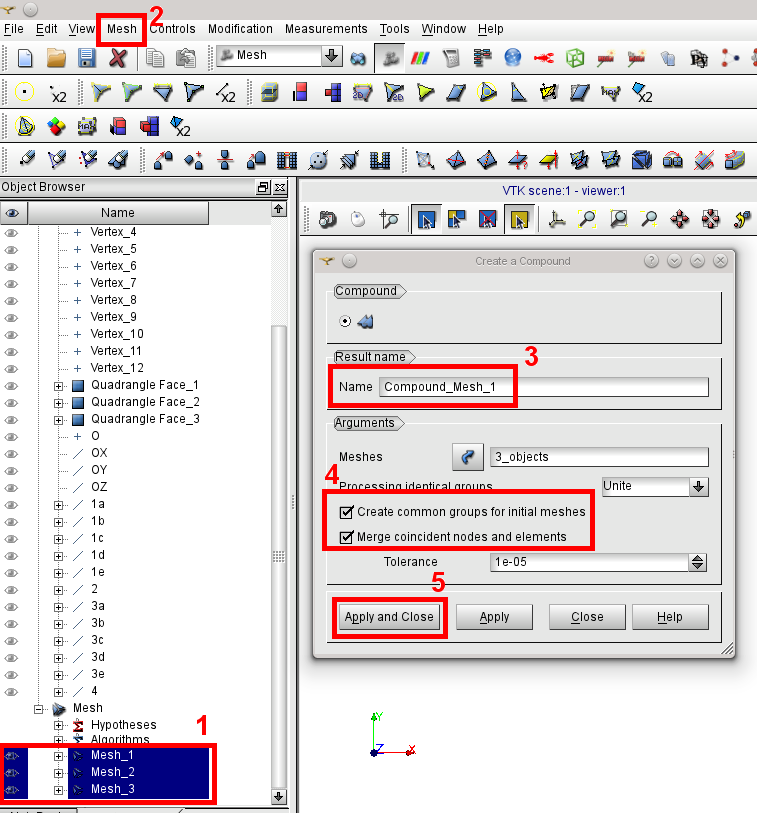
\includegraphics[scale=0.50]{figures/SalomeStep5.png}
\caption{Building a Compound Mesh.}
\label{fig:no3.2.1.13}
\end{center}
\end{figure}

In the \textbf{Object Browser} expand the \textbf{Compound\_Mesh\_1} and delete all groups except for the Material IDs in the \textbf{Groups of Faces} (Figure \ref{fig:no3.2.1.15}).
        
\begin{figure}[h!]
\begin{center}
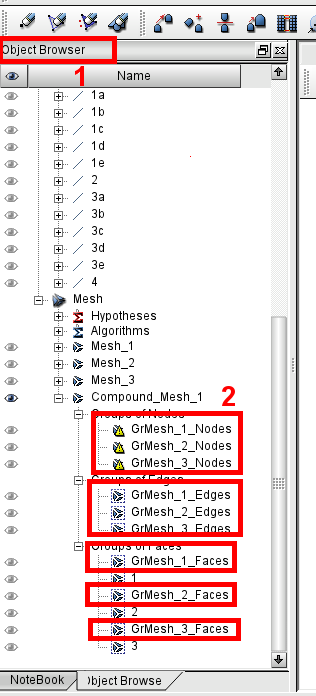
\includegraphics[scale=0.50]{figures/SalomeStep5b.png}
\caption{Deleting Unnecessary Groups.}
\label{fig:no3.2.1.15}
\end{center}
\end{figure}
          
The same technique as the above tip can be used to define the Boundary IDs by selecting them by hand. Another method that is easier for more complex shapes with finer meshes can be done as follows. Go back to \textbf{Geometry} and create lines around the Boundary. Like vertices this is done by going \textbf{New Entity} $\rightarrow$ \textbf{Basic} $\rightarrow$ \textbf{Line}. Change \textbf{Name} to whatever is easiest for you, I prefer to give them some name related to the Boundary ID they represent and use a letter afterwards if multiple lines represent the same Boundary ID. Select the vertices along the line, then select \textbf{Apply}. The vertice in Point 2 will then move to Point 1 and you can then continue this process in a clockwise or counter-clockwise direction. Once you reach the last line you can then select \textbf{Apply and Close} (Figure \ref{fig:no3.2.1.16}).
  
\begin{figure}[h!]
\begin{center}
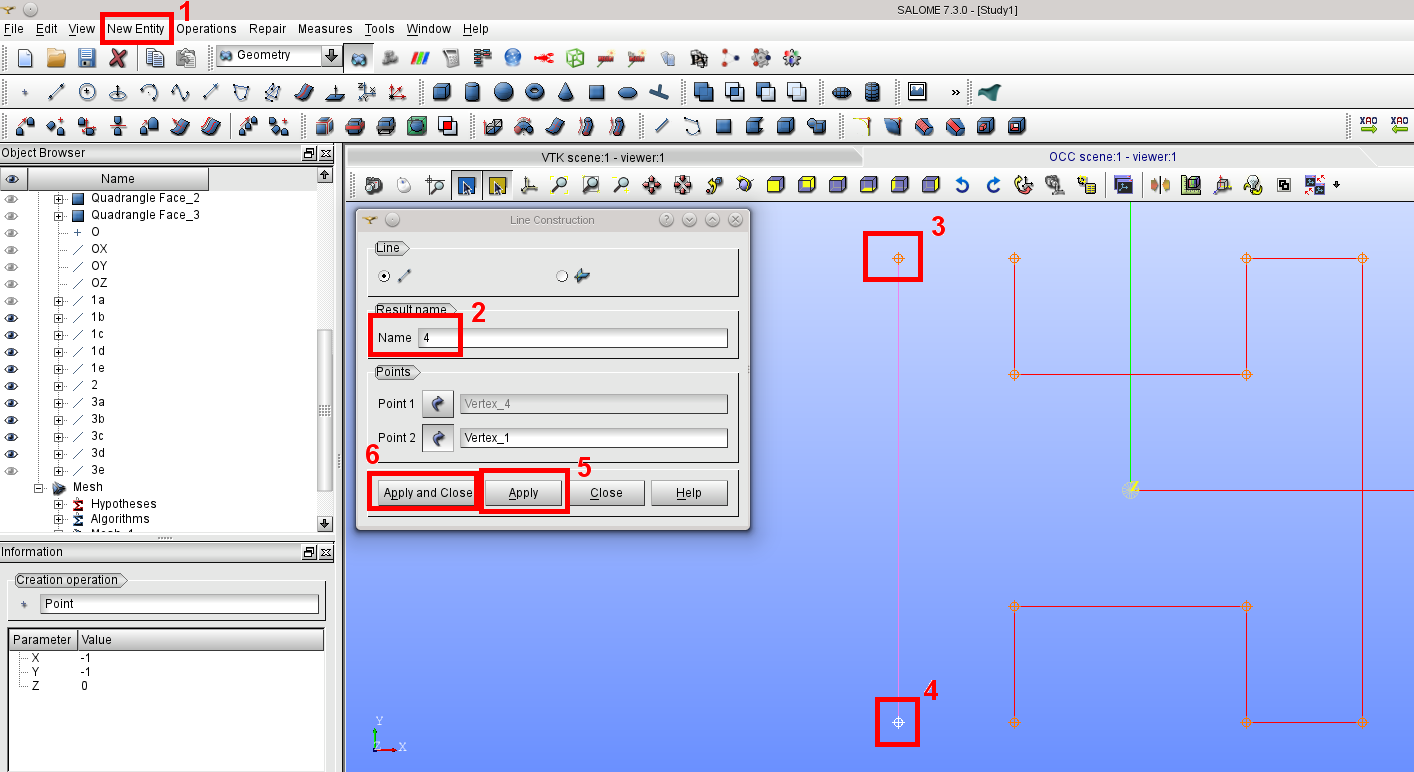
\includegraphics[scale=0.40]{figures/SalomeStep6.png}
\caption{Creating Lines for Use in Boundary ID Filter.}
\label{fig:no3.2.1.16}
\end{center}
\end{figure}

Back in \textbf{Mesh} right click the \textbf{Compound\_Mesh\_1} and select \textbf{Create Group}.  Select an \textbf{Element Type} of \textbf{Edge} and change the \textbf{Name} to the designated  Boundary ID. Select \textbf{Enable manual edition} and then select \textbf{Set Filter}.  In the case of Boundary ID 1 we have 5 lines so press \textbf{Add} 5 times then change   \textbf{Criterion} to \textbf{Belong to Geom}, \textbf{Binary} from \textbf{And} to \textbf{Or},  and for \textbf{Threshold value} select the empty square then select one of the lines from the  \textbf{Object Browser}. Once all the lines for the filter are set, select \textbf{Apply and Close}. Back in the \textbf{Create Group} window select \textbf{Add} and then \textbf{Apply and Close} (Figure \ref{fig:no3.2.1.17}). Repeat this process for each Boundary ID.
  
\begin{figure}[h!]
\begin{center}
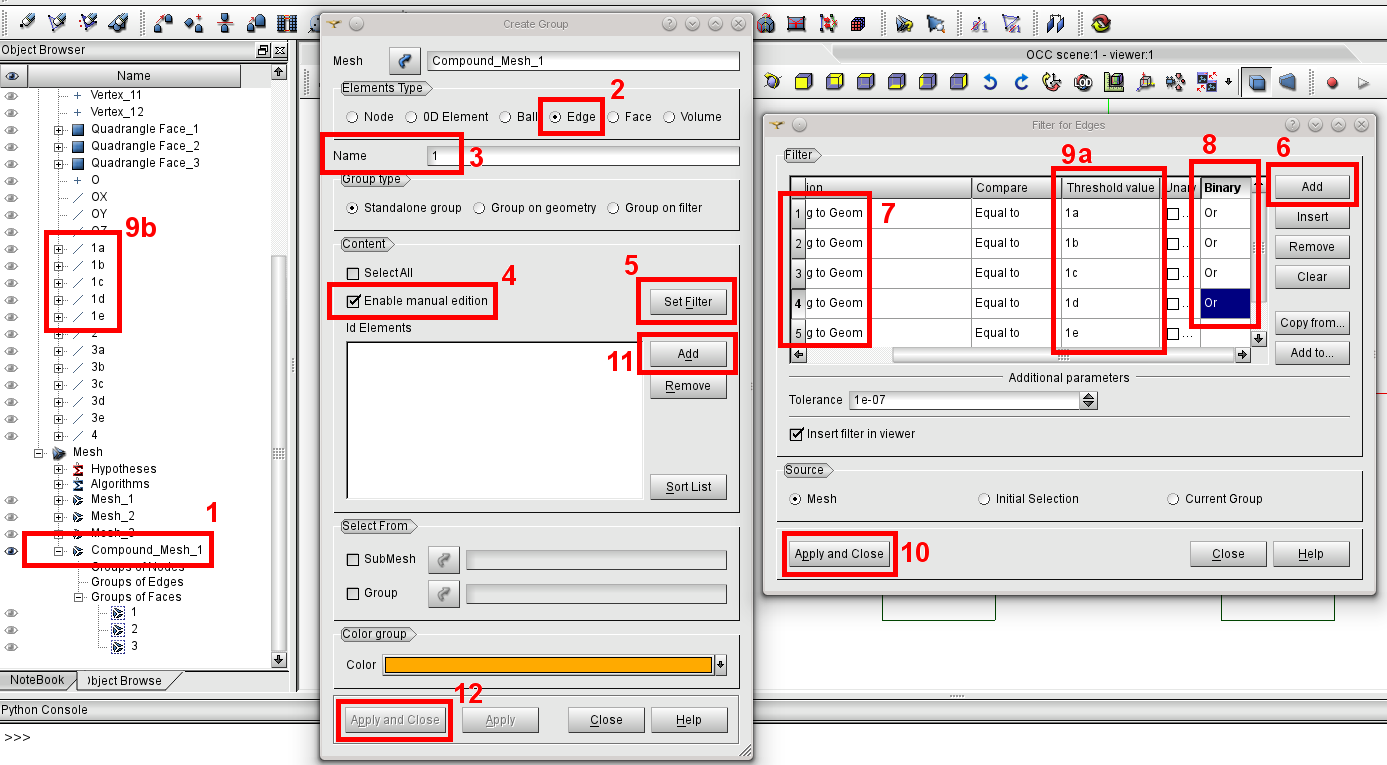
\includegraphics[scale=0.40]{figures/SalomeStep6b.png}
\caption{Creating a Boundary ID Filter.}
\label{fig:no3.2.1.17}
\end{center}
\end{figure}

\subsubsection{Removing internal edges}

Internal edges (and faces in 3D) are strictly prohibited by the OpenFCST architecture.  To see these internal edges, left click the Compound Mesh then right click the picture of it in the view. Then in \textbf{Numbering} select \textbf{Display Elements \#}. This will display all the edge and face numbers. As shown in Figure \ref{fig:no3.2.1.18}, it can be seen that lines 3, 4, 17, and 18 must be deleted. 
  
\begin{figure}[h!]
\begin{center}
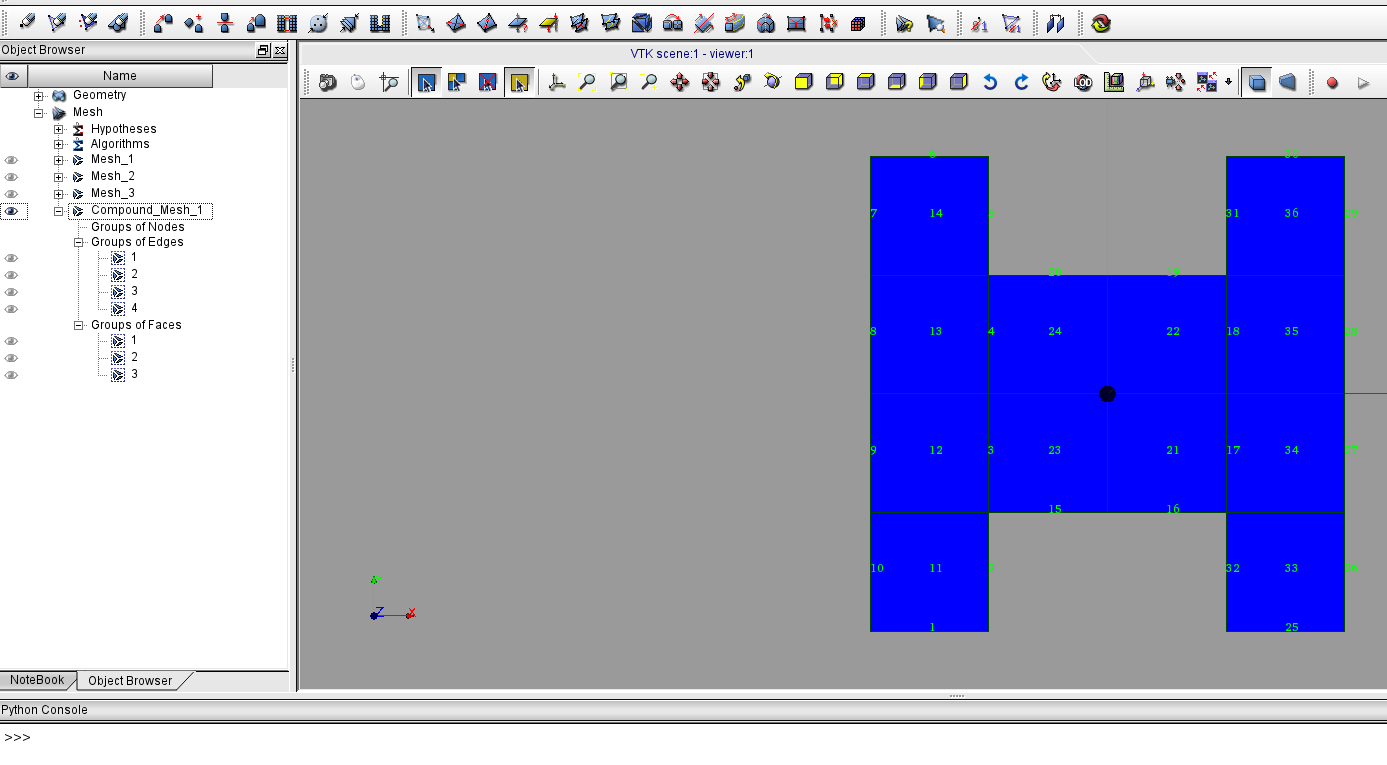
\includegraphics[scale=0.40]{figures/SalomeStep7.png}
\caption{Overview of the Mesh with Internal Edge Numbering (NOT allowed).}
\label{fig:no3.2.1.18}
\end{center}
\end{figure}
  
To manually remove these internal edges, in the toolbox select \textbf{Modification} $\rightarrow$ \textbf{Remove} $\rightarrow$ \textbf{Elements}. You can then either select the edge or enter the numbers and then select \textbf{Apply and Close}. This is rather easy in this simple project, but it can become cumbersome in more complex meshes. In openfcst/pre\_processing, there are two python scripts, RemoveInternalEdges.py and RemoveInternalFaces.py. In our case we need to open RemoveInternalEdges.py, change the mesh\_name on line 12 to the name of our Compound Mesh and save. Back in SALOME select \textbf{File} $\rightarrow$ \textbf{Load Script} select the RemoveInternalEdges.py, and it will automatically remove all internal edges.
  
\subsubsection{Exporting the mesh to UNV format}

Now the mesh can be exported to a UNV file. Right click the Compound Mesh in the \textbf{Object Browser}, then select \textbf{Export} $\rightarrow$ \textbf{UNV file}. Finally, save your mesh. Once we export the whole mesh into an UNV file, we can use it for the computational purposes (see the respective OpenFCST tutorial).

\textit{Tip:} Sometimes issues are caused by the first few lines of the UNV file when importing it to OpenFCST. To prevent this you can delete the first 17 lines of the UNV file so the file actually begins at line 18. The begining of these UNV files all look similar to the following:

\begin{lstlisting}
    -1
   164
         1  SI: Meter (newton)         2
    1.0000000000000000E+0    1.0000000000000000E+0    1.0000000000000000E+0
    2.7314999999999998E+2
    -1
    -1
  2420
         1
SMESH_Mesh
         1         0         0
Global Cartesian Coordinate System
    1.0000000000000000E+0    0.0000000000000000E+0    0.0000000000000000E+0
    0.0000000000000000E+0    1.0000000000000000E+0    0.0000000000000000E+0
    0.0000000000000000E+0    0.0000000000000000E+0    1.0000000000000000E+0
    0.0000000000000000E+0    0.0000000000000000E+0    0.0000000000000000E+0
    -1
    -1
  2411
  ...
\end{lstlisting}
  
%%======================================================
\section{SALOME meshing using python scripts}

%%=======
\subsection{Introduction}

The previous section discussed meshing in SALOME using the graphical user interface (GUI). This section will focus on creating and running scripts to create meshes and geometries. Reasons for using scripts 
instead of the GUI are as follows: improved repeatability of results, significant time saving due to automation, and removal of human error. Several Python scripts included in the pre\_processing
folder can be used to create various meshes of various geometries.

Meshing scripts are run through SALOME's text user interface (TUI). Loading scripts can be done simply via the File drop down menu, Load Script. Meshing scripts are written in Python programming language.
Python is a very popular general purpose high level programming language. Unlike C++, Python code is not precompiled, but interpreted at run time by a Python interpreter. Some key features
that make Python popular are its simple yet elegant syntax, dynamic typing, automatic memory management, and large selection of freely available libraries. If you are interested in
learning the Python programming language, we recommend \href{http://www.diveintopython.net/}{Dive Into Python}.

%%=======
\subsection{Scripting Examples}

\begin{lstlisting}[language=Python]
import smesh, geompy, SMESH
import SALOMEDS   
\end{lstlisting}

The above lines import the necessary SALOME packages that will be required to create geometries and meshes. \textit{smesh} is used to create python mesh objects,
\textit{geompy} is used for creating geometries. The other two packages contain constant flags. For more detail, please see the following resources:

\begin{enumerate}
 \item \href{http://docs.salome-platform.org/salome_6_5_0/gui/SMESH/smeshpy_doc/smesh_8py.html}{\textit{smesh} functions};
 \item \href{http://docs.salome-platform.org/salome_6_5_0/gui/GEOM/tui_basic_geom_objs_page.html}{\textit{geompy} documentation};
 \item \href{http://docs.salome-platform.org/salome_6_5_0/gui/SMESH/smeshpy_interface_page.html}{Salome TUI documentation}.
\end{enumerate}

The following simple example shows how to use geompy to create a simple geometry and then mesh it using smesh.

\begin{lstlisting}[language=Python]
def makeRectanglarMesh(self, width, height):

    #Create vertices to describe rectangle
    Vertex_1 = geompy.MakeVertex(dList[0], dList[1], dList[2])
    Vertex_2 = geompy.MakeVertex(dList[0] + width, dList[1], dList[2])
    Vertex_3 = geompy.MakeVertex(dList[0] + width, dList[1] + height, dList[2])
    Vertex_4 = geompy.MakeVertex(dList[0], dList[1] + height, dList[2])
    
    #Make rectangle geometries
    rect = geompy.MakeQuad4Vertices(Vertex_1, Vertex_2, Vertex_3, Vertex_4)
    
    #Create mesh object of rectangular geomtery
    Mesh_1 = smesh.Mesh(rect)
    
    #Set 1D meshing algorithm
    Regular_1D = Mesh_1.Segment()
    Local_Length_1 = Regular_1D.LocalLength(self.meshDensity)
    Local_Length_1.SetPrecision( 1e-07 )
    
    #Set 2D meshing algorithm
    Mesh_1.Quadrangle()
    
    #Compute and return
    Mesh_1.Compute()
    return Mesh_1 

\end{lstlisting}

The following is an example of modifying meshes and using mesh filters.

\begin{lstlisting}[language=Python]
def delInternalEdges(self):
    'This function deletes internal edges from self.compoundMesh'
    
    #Create a search filter to find free borders of the mesh
    search_filter = smesh.GetFilter(smesh.EDGE, smesh.FT_FreeBorders)
    external_edges = self.compoundMesh.GetIdsFromFilter(search_filter)
    
    #Get a list of all edges
    all_edges = self.compoundMesh.GetElementsByType(SMESH.EDGE)
    
    edges_to_remove = []
    
    #The difference between the external_edges list and all_edges list will be the internal edges.
    #The following loop iterates through the all_edges list, comparing it wil the external_edges list.
    
    for b in all_edges:
	if b in external_edges:
	    pass
	else:
	    #The edge is internal, add it to the list of items to be removed from the mesh
	    edge_to_remove.append(b)
    
    print "Removing internal edges:"
    print edges_to_remove
    
    #Remove the edges from the mesh
    self.compoundMesh.RemoveElements(edges_to_remove)
    
\end{lstlisting}        

When developing a new Python function for generating a geometry or mesh in SALOME one may obtain a rough solution by following these steps:

\begin{enumerate}
 \item open the SALOME GUI;
 \item perform the necessary steps using the GUI to generate the desired geometries and/or surfaces;
 \item use the ``Dump Study'' facility, accessed from the File menu, to produce a bulky but complete python program for the previously performed steps;
 \item refine the script to the desired form.
\end{enumerate}

This is a very good method for obtaining an initial coding solution or examples of correct code syntax and usage.

%%===============================================================
\section{Generating a VTK mesh using PythonFCST}

\subsection{Using the Python executable writeVTK.py}

PythonFCST comes equipped with a Python executable \textbf{writeVTK.py} which reads in a stack of tiff images and generates a Legacy Unstructured Grid file using the pixel values in the images as the material ids for the mesh. Before running \textbf{writeVTK.py}, it is important that OpenFCST is installed on the system and the OpenFCST environment variables are set using the \textbf{fcst\_env.sh} file in the FCST Install Directory (\verb!${FCST_DIR}!). To set the environment variables, type the following command in the Terminal (or Konsole) from \verb!${FCST_DIR}!:

\begin{lstlisting}[language=bash]
$ . fcst_env.sh
\end{lstlisting}

Once the environment variables have been set, the \textbf{writeVTK.py} should be available as a command line utility. To ensure that the environment variable has been set, the following command can be used:

\begin{lstlisting}[language=bash]
$ writeVTK.py -h
\end{lstlisting}

\noindent The above command generates the help documentation for the writeVTK.py:

\begin{lstlisting}[language=bash]
Usage: writeVTK.py [options]

Options:
-h, --help            show this help message and exit
-f FILE, --file=FILE  relative path of the images to be converted
-b BASENAME, --basename=BASENAME
                      basename of the image files. Default: 'Slice_'  would
                      mean images with name Slice_001 and so on
-n NUM                Number of images to be read. Default: 200
-o OUTPUT             Output file name. Default: test.vtk
-m MATERIAL, --material=MATERIAL
                      material id of the phase to be meshed. Default: 0
-v VOXEL, --voxel=VOXEL
                      voxel size as x y z
-e EXTENSION, --extension=EXTENSION
                      extension for the input files. Default is .tiff
\end{lstlisting}


In order to generate the mesh, the relative folder location from the current working directory for the images needs to be specified with the \verb!-f! identifier. The basename of the images refers to the name of the image without the numerical part and extension. For example, for images named \textbf{``Slice\_001.tiff''} to \textbf{``Slice\_100.tiff''} the basename would be \textbf{``Slice\_''}. The number of images to be read in is specified with the \verb!-n! identifier. Identifier \verb!-o! is used to specify the output file name. The voxel size, which is the dimension in cm per pixel in the X, Y, and Z directions, is specified with the \verb!-v! identifier. By default, the extension for the images is \textbf{``.tiff''}. If the images have a different extension, then they must be specified with the \verb!-e! identifier. Another important option is the material ID which can be specified with the \verb!-m! option. The material ID represents the pixel value for which the mesh should be generated. The default material ID is 0 which corresponds to the black color in a grey-scale image.

In the following example, we will generate a mesh from 10 images in the folder\\
\texttt{\${FCST\_DIR}/examples/microscale/3D\_Diffusion/images} while the current working directory is\\
\verb!${FCST_DIR}/examples/microscale/3D_Diffusion!:

\begin{lstlisting}[language=bash]
$ writeVTK.py -f images/ -b Slice_ -n 10 -o my_test.vtk -m 0 -v 1e-6 1e-6 1e-6 -e .tiff

==================================================
==================================================
=  Points and cells Created
=  Writing a VTK file
==================================================
Calculating Fitted Sphere Size Distribution
**************************************************
= Processing dataset
--------------------------------------------------
==================================================
= Calculate PSD
=  - Pore radius 1e-06
=  - Pore radius 1.1643739803e-06
=  - Pore radius 1.32874796059e-06
=  - Pore radius 1.49312194089e-06
=  - Pore radius 1.65749592118e-06
=  - Pore radius 1.82186990148e-06
=  - Pore radius 1.98624388177e-06
=  - Pore radius 2.15061786207e-06
=  - Pore radius 2.31499184237e-06
=  - Pore radius 2.47936582266e-06
=  - Pore radius 2.64373980296e-06
=  - Pore radius 2.80811378325e-06
=  - Pore radius 2.97248776355e-06
=  - Pore radius 3.13686174384e-06
=  - Pore radius 3.30123572414e-06
=  - Pore radius 3.46560970443e-06
=  - Pore radius 3.62998368473e-06
=  - Pore radius 3.79435766503e-06
=  - Pore radius 3.95873164532e-06
=  - Pore radius 4.12310562562e-06
= The file has been successfully written!
--------------------------------------------------
Phase with material id: 0  is represented by material id 0 in the mesh file:  my_test.vtk
time elapsed is  17.7439901829  seconds
\end{lstlisting}

If the command runs successfully, the above output will be displayed and the mesh file named \textbf{my\_test.vtk} will be written to the \verb!${FCST_DIR}/examples/microscale/3D_Diffusion! (which was the current working directory). In addition to generating the mesh, the code also calculates the local radius based on a sphere fitting algorithm~\cite{Sabharwal2016analysis} of the phase and stores it in the generated mesh which can be later used in OpenFCST to account for the local Knudsen effects in the diffusion simulations.

\subsection{Using the MESH module in PythonFCST}

For people who are familiar with Python, using the \textbf{PythonFCST.mesh} module might be another option to generate the mesh. The mesh module contains the Grid Generator class which generates the VTK mesh. The arguments to be supplied are a 3D numpy array (argument name: \verb!image!) and the output filename (argument name: \verb!filename!). This provides a bit more flexibility to use any 3D numpy array which might have been generated from any source rather than being limited to a stack of tiff images.

For the purpose of this example, we would deal with the same set of images as above. Let's use the \textbf{PythonFCST.mesh} module to generate the mesh. The code snippet below describes how to use it.

\begin{lstlisting}[language=Python]
#Initial imports for libraries and modules

import PythonFCST.mesh.PhaseGenerator as grid
from PIL import Image
import os
import numpy as np

#Defining variables to read in images; Omit this section if you already have a 3D array

foldername = "images"
basename = "Slice_"
num_images = 10
output = "my_test.vtk"
name=os.getcwd()+'/'+foldername+'/'+basename+'%.3d'
extension='.tiff'
tmp = []

#Looping over images and reading them
for i in range(num_images):
  filename=name%(i+1)+extension
  tmp.append(np.asarray(Image.open(filename),dtype=np.float))

#Generating the 3D numpy array
image=np.dstack(tmp)
image[image>0]=20   #changing all non-zero material ids to 20; assuming that pixel value of 0 was the one of interest

#Generating the VTK mesh using the Mesh module in PythonFCST
o=grid(image,output,material=0)
o.write()
\end{lstlisting}

The generated mesh file, \textbf{my\_test.vtk}, has the material ID 0 from the grey scale images extracted. Figures~\ref{fig:VTK_PythonFCST_pores} and~\ref{fig:VTK_PythonFCST_boundaries} show the results of the example code discussed above.

\begin{figure}[h]
\centering
%\captionsetup{justification=centering,margin=2cm}
\captionsetup{justification=centering}
\subfloat[]{%
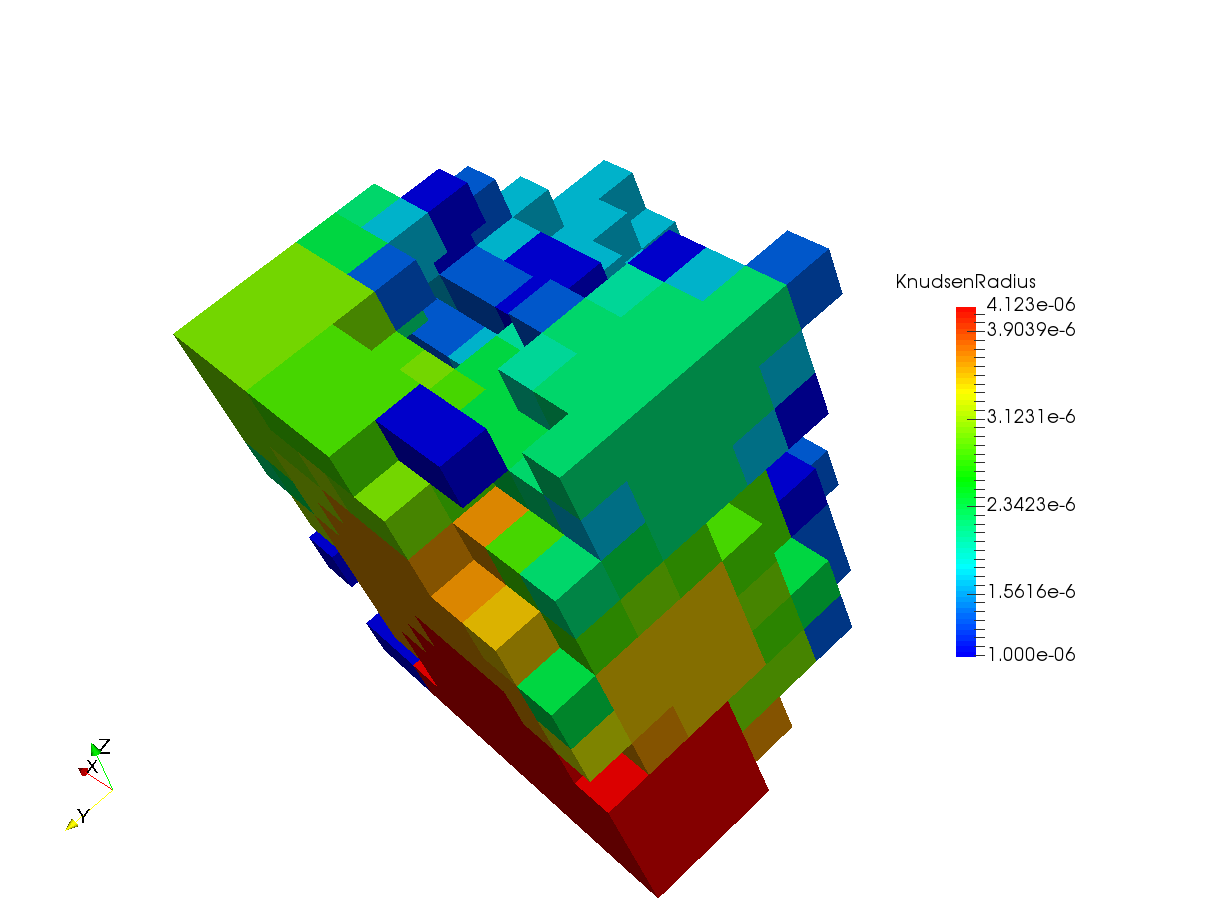
\includegraphics[width=0.45\linewidth]{figures/VTK_PythonFCST_pores.png}\label{fig:VTK_PythonFCST_pores}}
\quad
\subfloat[]{%
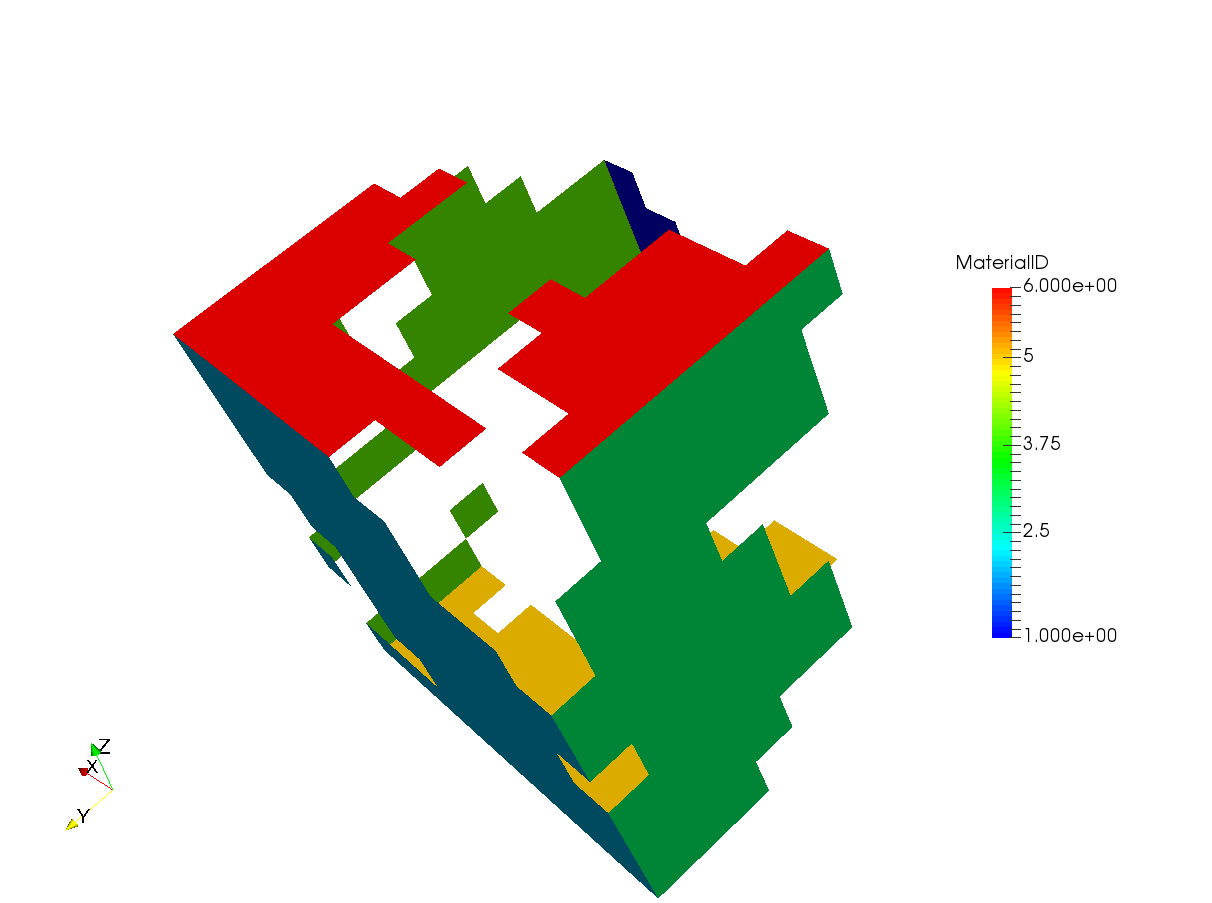
\includegraphics[width=0.45\linewidth]{figures/VTK_PythonFCST_boundaries.png}\label{fig:VTK_PythonFCST_boundaries}}
\caption{The resulting mesh of the pores (a) and representation of the boundary IDs 1-6 for the generated mesh (b).}
\label{fig:VTK_PythonFCST_pores_and_boundaries}
\end{figure}

\bigskip

\noindent\textbf{Note.} VTK files invert the X and Y axis from the images. Therefore, if the image had dimensions 20x30 in X and Y directions respectively, then the mesh will have dimensions 30x20 in the X and Y directions. By default, OpenFCST corrects for this so that the voxel sizes entered by user are in the true X and Y directions. Also, the boundary IDs are corrected so that 1-2 are boundary IDs in the true X direction and in the Y direction for the mesh as seen above.

The mesh can be further pre-processed using any of the filters in Paraview or Mayavi and can be written to a Legacy VTK file. This would still be compatible with the OpenFCST application.

%%===============================================================
%%===============================================================